\documentclass[1p]{elsarticle_modified}
%\bibliographystyle{elsarticle-num}

%\usepackage[colorlinks]{hyperref}
%\usepackage{abbrmath_seonhwa} %\Abb, \Ascr, \Acal ,\Abf, \Afrak
\usepackage{amsfonts}
\usepackage{amssymb}
\usepackage{amsmath}
\usepackage{amsthm}
\usepackage{scalefnt}
\usepackage{amsbsy}
\usepackage{kotex}
\usepackage{caption}
\usepackage{subfig}
\usepackage{color}
\usepackage{graphicx}
\usepackage{xcolor} %% white, black, red, green, blue, cyan, magenta, yellow
\usepackage{float}
\usepackage{setspace}
\usepackage{hyperref}

\usepackage{tikz}
\usetikzlibrary{arrows}

\usepackage{multirow}
\usepackage{array} % fixed length table
\usepackage{hhline}

%%%%%%%%%%%%%%%%%%%%%
\makeatletter
\renewcommand*\env@matrix[1][\arraystretch]{%
	\edef\arraystretch{#1}%
	\hskip -\arraycolsep
	\let\@ifnextchar\new@ifnextchar
	\array{*\c@MaxMatrixCols c}}
\makeatother %https://tex.stackexchange.com/questions/14071/how-can-i-increase-the-line-spacing-in-a-matrix
%%%%%%%%%%%%%%%

\usepackage[normalem]{ulem}

\newcommand{\msout}[1]{\ifmmode\text{\sout{\ensuremath{#1}}}\else\sout{#1}\fi}
%SOURCE: \msout is \stkout macro in https://tex.stackexchange.com/questions/20609/strikeout-in-math-mode

\newcommand{\cancel}[1]{
	\ifmmode
	{\color{red}\msout{#1}}
	\else
	{\color{red}\sout{#1}}
	\fi
}

\newcommand{\add}[1]{
	{\color{blue}\uwave{#1}}
}

\newcommand{\replace}[2]{
	\ifmmode
	{\color{red}\msout{#1}}{\color{blue}\uwave{#2}}
	\else
	{\color{red}\sout{#1}}{\color{blue}\uwave{#2}}
	\fi
}

\newcommand{\Sol}{\mathcal{S}} %segment
\newcommand{\D}{D} %diagram
\newcommand{\A}{\mathcal{A}} %arc


%%%%%%%%%%%%%%%%%%%%%%%%%%%%%5 test

\def\sl{\operatorname{\textup{SL}}(2,\Cbb)}
\def\psl{\operatorname{\textup{PSL}}(2,\Cbb)}
\def\quan{\mkern 1mu \triangleright \mkern 1mu}

\theoremstyle{definition}
\newtheorem{thm}{Theorem}[section]
\newtheorem{prop}[thm]{Proposition}
\newtheorem{lem}[thm]{Lemma}
\newtheorem{ques}[thm]{Question}
\newtheorem{cor}[thm]{Corollary}
\newtheorem{defn}[thm]{Definition}
\newtheorem{exam}[thm]{Example}
\newtheorem{rmk}[thm]{Remark}
\newtheorem{alg}[thm]{Algorithm}

\newcommand{\I}{\sqrt{-1}}
\begin{document}

%\begin{frontmatter}
%
%\title{Boundary parabolic representations of knots up to 8 crossings}
%
%%% Group authors per affiliation:
%\author{Yunhi Cho} 
%\address{Department of Mathematics, University of Seoul, Seoul, Korea}
%\ead{yhcho@uos.ac.kr}
%
%
%\author{Seonhwa Kim} %\fnref{s_kim}}
%\address{Center for Geometry and Physics, Institute for Basic Science, Pohang, 37673, Korea}
%\ead{ryeona17@ibs.re.kr}
%
%\author{Hyuk Kim}
%\address{Department of Mathematical Sciences, Seoul National University, Seoul 08826, Korea}
%\ead{hyukkim@snu.ac.kr}
%
%\author{Seokbeom Yoon}
%\address{Department of Mathematical Sciences, Seoul National University, Seoul, 08826,  Korea}
%\ead{sbyoon15@snu.ac.kr}
%
%\begin{abstract}
%We find all boundary parabolic representation of knots up to 8 crossings.
%
%\end{abstract}
%\begin{keyword}
%    \MSC[2010] 57M25 
%\end{keyword}
%
%\end{frontmatter}

%\linenumbers
%\tableofcontents
%
\newcommand\colored[1]{\textcolor{white}{\rule[-0.35ex]{0.8em}{1.4ex}}\kern-0.8em\color{red} #1}%
%\newcommand\colored[1]{\textcolor{white}{ #1}\kern-2.17ex	\textcolor{white}{ #1}\kern-1.81ex	\textcolor{white}{ #1}\kern-2.15ex\color{red}#1	}

{\Large $\underline{12n_{0607}~(K12n_{0607})}$}

\setlength{\tabcolsep}{10pt}
\renewcommand{\arraystretch}{1.6}
\vspace{1cm}\begin{tabular}{m{100pt}>{\centering\arraybackslash}m{274pt}}
\multirow{5}{120pt}{
	\centering
	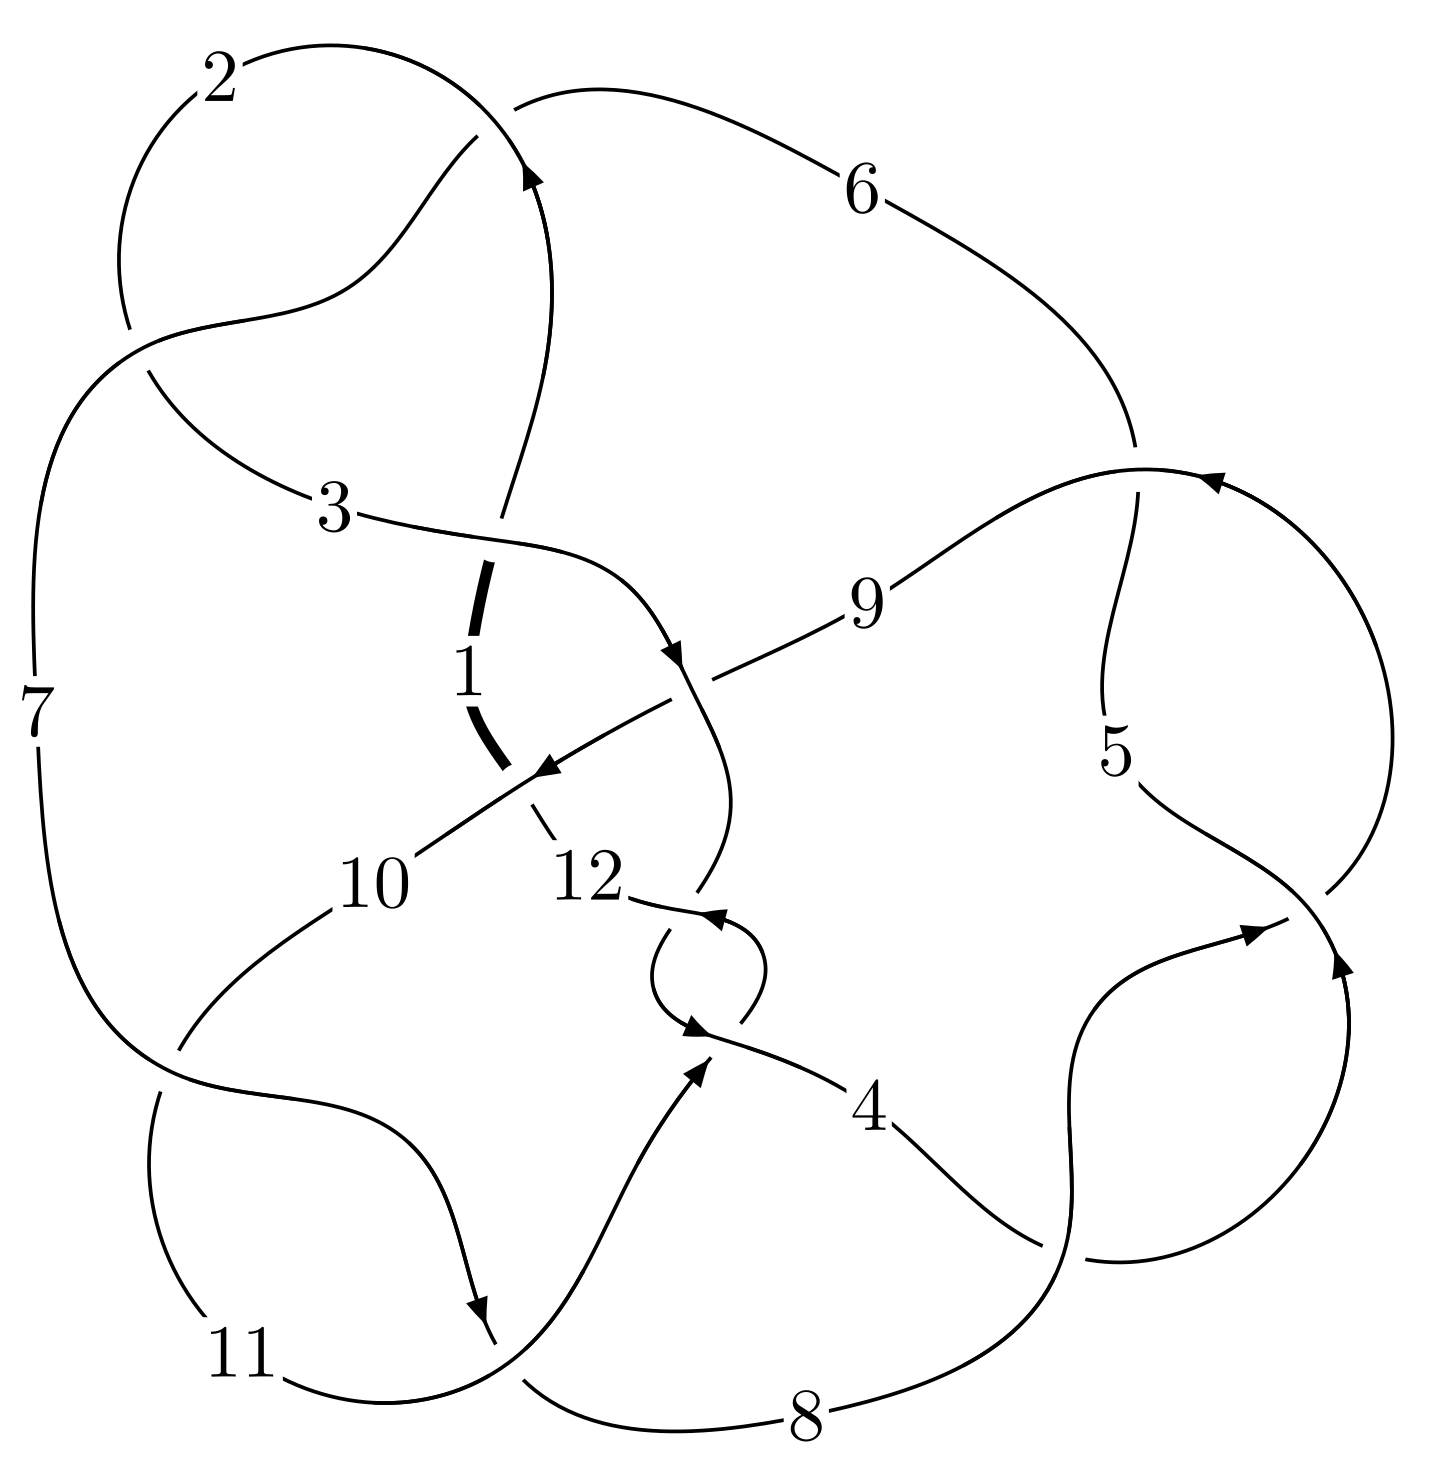
\includegraphics[width=112pt]{../../../GIT/diagram.site/Diagrams/png/2696_12n_0607.png}\\
\ \ \ A knot diagram\footnotemark}&
\allowdisplaybreaks
\textbf{Linearized knot diagam} \\
\cline{2-2}
 &
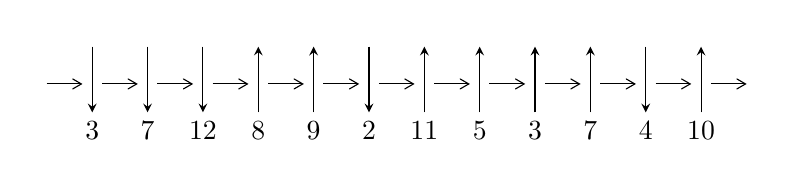
\begin{tikzpicture}[x=20pt, y=17pt]
	% nodes
	\node (C0) at (0, 0) {};
	\node (C1) at (1, 0) {};
	\node (C1U) at (1, +1) {};
	\node (C1D) at (1, -1) {3};

	\node (C2) at (2, 0) {};
	\node (C2U) at (2, +1) {};
	\node (C2D) at (2, -1) {7};

	\node (C3) at (3, 0) {};
	\node (C3U) at (3, +1) {};
	\node (C3D) at (3, -1) {12};

	\node (C4) at (4, 0) {};
	\node (C4U) at (4, +1) {};
	\node (C4D) at (4, -1) {8};

	\node (C5) at (5, 0) {};
	\node (C5U) at (5, +1) {};
	\node (C5D) at (5, -1) {9};

	\node (C6) at (6, 0) {};
	\node (C6U) at (6, +1) {};
	\node (C6D) at (6, -1) {2};

	\node (C7) at (7, 0) {};
	\node (C7U) at (7, +1) {};
	\node (C7D) at (7, -1) {11};

	\node (C8) at (8, 0) {};
	\node (C8U) at (8, +1) {};
	\node (C8D) at (8, -1) {5};

	\node (C9) at (9, 0) {};
	\node (C9U) at (9, +1) {};
	\node (C9D) at (9, -1) {3};

	\node (C10) at (10, 0) {};
	\node (C10U) at (10, +1) {};
	\node (C10D) at (10, -1) {7};

	\node (C11) at (11, 0) {};
	\node (C11U) at (11, +1) {};
	\node (C11D) at (11, -1) {4};

	\node (C12) at (12, 0) {};
	\node (C12U) at (12, +1) {};
	\node (C12D) at (12, -1) {10};
	\node (C13) at (13, 0) {};

	% arrows
	\draw[->,>={angle 60}]
	(C0) edge (C1) (C1) edge (C2) (C2) edge (C3) (C3) edge (C4) (C4) edge (C5) (C5) edge (C6) (C6) edge (C7) (C7) edge (C8) (C8) edge (C9) (C9) edge (C10) (C10) edge (C11) (C11) edge (C12) (C12) edge (C13) ;	\draw[->,>=stealth]
	(C1U) edge (C1D) (C2U) edge (C2D) (C3U) edge (C3D) (C4D) edge (C4U) (C5D) edge (C5U) (C6U) edge (C6D) (C7D) edge (C7U) (C8D) edge (C8U) (C9D) edge (C9U) (C10D) edge (C10U) (C11U) edge (C11D) (C12D) edge (C12U) ;
	\end{tikzpicture} \\
\hhline{~~} \\& 
\textbf{Solving Sequence} \\ \cline{2-2} 
 &
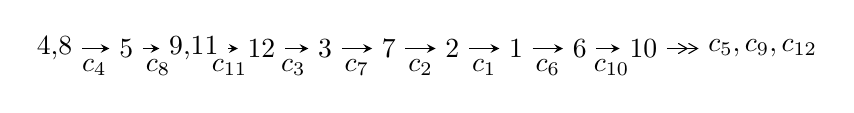
\begin{tikzpicture}[x=23pt, y=7pt]
	% node
	\node (A0) at (-1/8, 0) {4,8};
	\node (A1) at (1, 0) {5};
	\node (A2) at (33/16, 0) {9,11};
	\node (A3) at (25/8, 0) {12};
	\node (A4) at (33/8, 0) {3};
	\node (A5) at (41/8, 0) {7};
	\node (A6) at (49/8, 0) {2};
	\node (A7) at (57/8, 0) {1};
	\node (A8) at (65/8, 0) {6};
	\node (A9) at (73/8, 0) {10};
	\node (C1) at (1/2, -1) {$c_{4}$};
	\node (C2) at (3/2, -1) {$c_{8}$};
	\node (C3) at (21/8, -1) {$c_{11}$};
	\node (C4) at (29/8, -1) {$c_{3}$};
	\node (C5) at (37/8, -1) {$c_{7}$};
	\node (C6) at (45/8, -1) {$c_{2}$};
	\node (C7) at (53/8, -1) {$c_{1}$};
	\node (C8) at (61/8, -1) {$c_{6}$};
	\node (C9) at (69/8, -1) {$c_{10}$};
	\node (A10) at (11, 0) {$c_{5},c_{9},c_{12}$};

	% edge
	\draw[->,>=stealth]	
	(A0) edge (A1) (A1) edge (A2) (A2) edge (A3) (A3) edge (A4) (A4) edge (A5) (A5) edge (A6) (A6) edge (A7) (A7) edge (A8) (A8) edge (A9) ;
	\draw[->>,>={angle 60}]	
	(A9) edge (A10);
\end{tikzpicture} \\ 

\end{tabular} \\

\footnotetext{
The image of knot diagram is generated by the software ``\textbf{Draw programme}" developed by Andrew Bartholomew(\url{http://www.layer8.co.uk/maths/draw/index.htm\#Running-draw}), where we modified some parts for our purpose(\url{https://github.com/CATsTAILs/LinksPainter}).
}\phantom \\ \newline 
\centering \textbf{Ideals for irreducible components\footnotemark of $X_{\text{par}}$} 
 
\begin{align*}
I^u_{1}&=\langle 
-3.98483\times10^{51} u^{43}-7.92706\times10^{51} u^{42}+\cdots+1.21780\times10^{52} b+9.50729\times10^{52},\\
\phantom{I^u_{1}}&\phantom{= \langle  }-6.39484\times10^{51} u^{43}-5.55868\times10^{51} u^{42}+\cdots+3.53162\times10^{53} a+2.88768\times10^{53},\\
\phantom{I^u_{1}}&\phantom{= \langle  }u^{44}+3 u^{43}+\cdots-36 u-29\rangle \\
I^u_{2}&=\langle 
u^{13}- u^{12}-7 u^{11}+7 u^{10}+18 u^9-18 u^8-20 u^7+18 u^6+10 u^5-2 u^4-5 u^3-4 u^2+b+2 u+1,\\
\phantom{I^u_{2}}&\phantom{= \langle  }- u^{14}+2 u^{13}+7 u^{12}-16 u^{11}-17 u^{10}+50 u^9+13 u^8-74 u^7+6 u^6+50 u^5-6 u^4-12 u^3-6 u^2+a+5,\\
\phantom{I^u_{2}}&\phantom{= \langle  }u^{15}-2 u^{14}-7 u^{13}+16 u^{12}+17 u^{11}-50 u^{10}-13 u^9+74 u^8-6 u^7-50 u^6+6 u^5+12 u^4+6 u^3+u^2-5 u-1\rangle \\
\\
\end{align*}
\raggedright * 2 irreducible components of $\dim_{\mathbb{C}}=0$, with total 59 representations.\\
\footnotetext{All coefficients of polynomials are rational numbers. But the coefficients are sometimes approximated in decimal forms when there is not enough margin.}
\newpage
\renewcommand{\arraystretch}{1}
\centering \section*{I. $I^u_{1}= \langle -3.98\times10^{51} u^{43}-7.93\times10^{51} u^{42}+\cdots+1.22\times10^{52} b+9.51\times10^{52},\;-6.39\times10^{51} u^{43}-5.56\times10^{51} u^{42}+\cdots+3.53\times10^{53} a+2.89\times10^{53},\;u^{44}+3 u^{43}+\cdots-36 u-29 \rangle$}
\flushleft \textbf{(i) Arc colorings}\\
\begin{tabular}{m{7pt} m{180pt} m{7pt} m{180pt} }
\flushright $a_{4}=$&$\begin{pmatrix}1\\0\end{pmatrix}$ \\
\flushright $a_{8}=$&$\begin{pmatrix}0\\u\end{pmatrix}$ \\
\flushright $a_{5}=$&$\begin{pmatrix}1\\- u^2\end{pmatrix}$ \\
\flushright $a_{9}=$&$\begin{pmatrix}u\\- u^3+u\end{pmatrix}$ \\
\flushright $a_{11}=$&$\begin{pmatrix}0.0181074 u^{43}+0.0157397 u^{42}+\cdots-7.01705 u-0.817663\\0.327216 u^{43}+0.650933 u^{42}+\cdots-4.17363 u-7.80693\end{pmatrix}$ \\
\flushright $a_{12}=$&$\begin{pmatrix}-0.309108 u^{43}-0.635193 u^{42}+\cdots-2.84342 u+6.98927\\0.327216 u^{43}+0.650933 u^{42}+\cdots-4.17363 u-7.80693\end{pmatrix}$ \\
\flushright $a_{3}=$&$\begin{pmatrix}0.518338 u^{43}+1.03102 u^{42}+\cdots-15.2327 u-13.7592\\-0.303941 u^{43}-0.580963 u^{42}+\cdots+5.51276 u+8.99431\end{pmatrix}$ \\
\flushright $a_{7}=$&$\begin{pmatrix}0.549754 u^{43}+1.13751 u^{42}+\cdots-14.1047 u-14.7839\\-0.193131 u^{43}-0.327791 u^{42}+\cdots+2.95340 u+6.21753\end{pmatrix}$ \\
\flushright $a_{2}=$&$\begin{pmatrix}0.232795 u^{43}+0.476323 u^{42}+\cdots+3.84795 u-8.66991\\-0.371791 u^{43}-0.806245 u^{42}+\cdots+1.40362 u+10.8222\end{pmatrix}$ \\
\flushright $a_{1}=$&$\begin{pmatrix}-0.350328 u^{43}-0.903767 u^{42}+\cdots+29.3966 u+10.2617\\-0.431119 u^{43}-0.755303 u^{42}+\cdots-1.45502 u+5.30649\end{pmatrix}$ \\
\flushright $a_{6}=$&$\begin{pmatrix}- u^2+1\\u^4-2 u^2\end{pmatrix}$ \\
\flushright $a_{10}=$&$\begin{pmatrix}-0.00534609 u^{43}-0.0637310 u^{42}+\cdots-3.23886 u-5.04605\\-0.0972752 u^{43}-0.0928284 u^{42}+\cdots-4.57450 u+2.98741\end{pmatrix}$\\&\end{tabular}
\flushleft \textbf{(ii) Obstruction class $= -1$}\\~\\
\flushleft \textbf{(iii) Cusp Shapes $= -0.277792 u^{43}-0.610725 u^{42}+\cdots+9.19368 u+15.3613$}\\~\\
\newpage\renewcommand{\arraystretch}{1}
\flushleft \textbf{(iv) u-Polynomials at the component}\newline \\
\begin{tabular}{m{50pt}|m{274pt}}
Crossings & \hspace{64pt}u-Polynomials at each crossing \\
\hline $$\begin{aligned}c_{1}\end{aligned}$$&$\begin{aligned}
&u^{44}+54 u^{43}+\cdots+157 u+1
\end{aligned}$\\
\hline $$\begin{aligned}c_{2},c_{6}\end{aligned}$$&$\begin{aligned}
&u^{44}-2 u^{43}+\cdots+3 u-1
\end{aligned}$\\
\hline $$\begin{aligned}c_{3},c_{11}\end{aligned}$$&$\begin{aligned}
&u^{44}-3 u^{43}+\cdots-25 u+1
\end{aligned}$\\
\hline $$\begin{aligned}c_{4},c_{5},c_{8}\end{aligned}$$&$\begin{aligned}
&u^{44}-3 u^{43}+\cdots+36 u-29
\end{aligned}$\\
\hline $$\begin{aligned}c_{7},c_{10}\end{aligned}$$&$\begin{aligned}
&u^{44}-4 u^{43}+\cdots+2004 u-563
\end{aligned}$\\
\hline $$\begin{aligned}c_{9}\end{aligned}$$&$\begin{aligned}
&u^{44}-2 u^{43}+\cdots+2091 u-389
\end{aligned}$\\
\hline $$\begin{aligned}c_{12}\end{aligned}$$&$\begin{aligned}
&u^{44}+u^{43}+\cdots+1354 u-1081
\end{aligned}$\\
\hline
\end{tabular}\\~\\
\newpage\renewcommand{\arraystretch}{1}
\flushleft \textbf{(v) Riley Polynomials at the component}\newline \\
\begin{tabular}{m{50pt}|m{274pt}}
Crossings & \hspace{64pt}Riley Polynomials at each crossing \\
\hline $$\begin{aligned}c_{1}\end{aligned}$$&$\begin{aligned}
&y^{44}-114 y^{43}+\cdots-6565 y+1
\end{aligned}$\\
\hline $$\begin{aligned}c_{2},c_{6}\end{aligned}$$&$\begin{aligned}
&y^{44}-54 y^{43}+\cdots-157 y+1
\end{aligned}$\\
\hline $$\begin{aligned}c_{3},c_{11}\end{aligned}$$&$\begin{aligned}
&y^{44}+43 y^{43}+\cdots-415 y+1
\end{aligned}$\\
\hline $$\begin{aligned}c_{4},c_{5},c_{8}\end{aligned}$$&$\begin{aligned}
&y^{44}-43 y^{43}+\cdots+154 y+841
\end{aligned}$\\
\hline $$\begin{aligned}c_{7},c_{10}\end{aligned}$$&$\begin{aligned}
&y^{44}-26 y^{43}+\cdots-2861866 y+316969
\end{aligned}$\\
\hline $$\begin{aligned}c_{9}\end{aligned}$$&$\begin{aligned}
&y^{44}+54 y^{43}+\cdots+12410735 y+151321
\end{aligned}$\\
\hline $$\begin{aligned}c_{12}\end{aligned}$$&$\begin{aligned}
&y^{44}+49 y^{43}+\cdots+24190678 y+1168561
\end{aligned}$\\
\hline
\end{tabular}\\~\\
\newpage\flushleft \textbf{(vi) Complex Volumes and Cusp Shapes}
$$\begin{array}{c|c|c}  
\text{Solutions to }I^u_{1}& \I (\text{vol} + \sqrt{-1}CS) & \text{Cusp shape}\\
 \hline 
\begin{aligned}
u &= \phantom{-}0.232314 + 0.891394 I \\
a &= -1.182840 + 0.641241 I \\
b &= -0.785573 + 0.181213 I\end{aligned}
 & -9.31236 + 3.20269 I & -1.63968 - 3.08905 I \\ \hline\begin{aligned}
u &= \phantom{-}0.232314 - 0.891394 I \\
a &= -1.182840 - 0.641241 I \\
b &= -0.785573 - 0.181213 I\end{aligned}
 & -9.31236 - 3.20269 I & -1.63968 + 3.08905 I \\ \hline\begin{aligned}
u &= -0.421682 + 0.772572 I \\
a &= -0.86640 - 1.32108 I \\
b &= \phantom{-}0.027933 - 1.313490 I\end{aligned}
 & \phantom{-}4.97162 + 0.16549 I & \phantom{-}5.68850 + 0.34807 I \\ \hline\begin{aligned}
u &= -0.421682 - 0.772572 I \\
a &= -0.86640 + 1.32108 I \\
b &= \phantom{-}0.027933 + 1.313490 I\end{aligned}
 & \phantom{-}4.97162 - 0.16549 I & \phantom{-}5.68850 - 0.34807 I \\ \hline\begin{aligned}
u &= -0.837269 + 0.017279 I \\
a &= -0.688236 - 0.510031 I \\
b &= \phantom{-}0.052866 + 0.391971 I\end{aligned}
 & \phantom{-}1.359070 + 0.099848 I & \phantom{-}6.44713 + 0.44768 I \\ \hline\begin{aligned}
u &= -0.837269 - 0.017279 I \\
a &= -0.688236 + 0.510031 I \\
b &= \phantom{-}0.052866 - 0.391971 I\end{aligned}
 & \phantom{-}1.359070 - 0.099848 I & \phantom{-}6.44713 - 0.44768 I \\ \hline\begin{aligned}
u &= -1.16381\phantom{ +0.000000I} \\
a &= \phantom{-}1.26734\phantom{ +0.000000I} \\
b &= \phantom{-}0.816752\phantom{ +0.000000I}\end{aligned}
 & \phantom{-}2.85076\phantom{ +0.000000I} & \phantom{-}2.72130\phantom{ +0.000000I} \\ \hline\begin{aligned}
u &= -1.187230 + 0.325824 I \\
a &= \phantom{-}1.367400 + 0.224408 I \\
b &= \phantom{-}0.332131 + 1.373840 I\end{aligned}
 & \phantom{-}7.30043 - 4.16721 I & \phantom{-}6.35771 + 3.21063 I \\ \hline\begin{aligned}
u &= -1.187230 - 0.325824 I \\
a &= \phantom{-}1.367400 - 0.224408 I \\
b &= \phantom{-}0.332131 - 1.373840 I\end{aligned}
 & \phantom{-}7.30043 + 4.16721 I & \phantom{-}6.35771 - 3.21063 I \\ \hline\begin{aligned}
u &= \phantom{-}1.229270 + 0.131786 I \\
a &= \phantom{-}0.802568 + 0.161525 I \\
b &= \phantom{-}0.892070 - 0.665689 I\end{aligned}
 & \phantom{-}2.18790 + 3.06008 I & \phantom{-}7.00945 - 4.71003 I\\
 \hline 
 \end{array}$$\newpage$$\begin{array}{c|c|c}  
\text{Solutions to }I^u_{1}& \I (\text{vol} + \sqrt{-1}CS) & \text{Cusp shape}\\
 \hline 
\begin{aligned}
u &= \phantom{-}1.229270 - 0.131786 I \\
a &= \phantom{-}0.802568 - 0.161525 I \\
b &= \phantom{-}0.892070 + 0.665689 I\end{aligned}
 & \phantom{-}2.18790 - 3.06008 I & \phantom{-}7.00945 + 4.71003 I \\ \hline\begin{aligned}
u &= -0.132670 + 0.748244 I \\
a &= \phantom{-}0.413490 + 1.238040 I \\
b &= \phantom{-}0.14531 + 1.46229 I\end{aligned}
 & \phantom{-}4.65271 - 3.21249 I & \phantom{-}2.19622 + 5.43824 I \\ \hline\begin{aligned}
u &= -0.132670 - 0.748244 I \\
a &= \phantom{-}0.413490 - 1.238040 I \\
b &= \phantom{-}0.14531 - 1.46229 I\end{aligned}
 & \phantom{-}4.65271 + 3.21249 I & \phantom{-}2.19622 - 5.43824 I \\ \hline\begin{aligned}
u &= \phantom{-}0.413623 + 1.194950 I \\
a &= -0.734599 + 0.755593 I \\
b &= -0.29763 + 1.39048 I\end{aligned}
 & -4.29060 + 7.07615 I & \phantom{-}2.00000 - 4.71324 I \\ \hline\begin{aligned}
u &= \phantom{-}0.413623 - 1.194950 I \\
a &= -0.734599 - 0.755593 I \\
b &= -0.29763 - 1.39048 I\end{aligned}
 & -4.29060 - 7.07615 I & \phantom{-}2.00000 + 4.71324 I \\ \hline\begin{aligned}
u &= \phantom{-}1.150740 + 0.556416 I \\
a &= \phantom{-}0.032760 - 0.925047 I \\
b &= -0.328510 - 0.006839 I\end{aligned}
 & -6.59118 + 1.93121 I & \phantom{-0.000000 } 0 \\ \hline\begin{aligned}
u &= \phantom{-}1.150740 - 0.556416 I \\
a &= \phantom{-}0.032760 + 0.925047 I \\
b &= -0.328510 + 0.006839 I\end{aligned}
 & -6.59118 - 1.93121 I & \phantom{-0.000000 } 0 \\ \hline\begin{aligned}
u &= -1.303890 + 0.194858 I \\
a &= -0.855836 + 0.581357 I \\
b &= -0.03406 - 1.56374 I\end{aligned}
 & \phantom{-}8.41843 - 0.01026 I & \phantom{-0.000000 } 0 \\ \hline\begin{aligned}
u &= -1.303890 - 0.194858 I \\
a &= -0.855836 - 0.581357 I \\
b &= -0.03406 + 1.56374 I\end{aligned}
 & \phantom{-}8.41843 + 0.01026 I & \phantom{-0.000000 } 0 \\ \hline\begin{aligned}
u &= \phantom{-}1.355820 + 0.181971 I \\
a &= \phantom{-}0.18635 - 1.43687 I \\
b &= -0.110848 + 1.367110 I\end{aligned}
 & -2.05757 + 3.46602 I & \phantom{-0.000000 } 0\\
 \hline 
 \end{array}$$\newpage$$\begin{array}{c|c|c}  
\text{Solutions to }I^u_{1}& \I (\text{vol} + \sqrt{-1}CS) & \text{Cusp shape}\\
 \hline 
\begin{aligned}
u &= \phantom{-}1.355820 - 0.181971 I \\
a &= \phantom{-}0.18635 + 1.43687 I \\
b &= -0.110848 - 1.367110 I\end{aligned}
 & -2.05757 - 3.46602 I & \phantom{-0.000000 } 0 \\ \hline\begin{aligned}
u &= -1.363940 + 0.224481 I \\
a &= -0.752199 - 0.014028 I \\
b &= -0.777456 + 1.110380 I\end{aligned}
 & -1.75499 - 1.31745 I & \phantom{-0.000000 } 0 \\ \hline\begin{aligned}
u &= -1.363940 - 0.224481 I \\
a &= -0.752199 + 0.014028 I \\
b &= -0.777456 - 1.110380 I\end{aligned}
 & -1.75499 + 1.31745 I & \phantom{-0.000000 } 0 \\ \hline\begin{aligned}
u &= \phantom{-}1.41075 + 0.33605 I \\
a &= \phantom{-}1.010620 + 0.344192 I \\
b &= \phantom{-}0.26866 - 1.59656 I\end{aligned}
 & \phantom{-}9.67423 + 7.25773 I & \phantom{-0.000000 } 0 \\ \hline\begin{aligned}
u &= \phantom{-}1.41075 - 0.33605 I \\
a &= \phantom{-}1.010620 - 0.344192 I \\
b &= \phantom{-}0.26866 + 1.59656 I\end{aligned}
 & \phantom{-}9.67423 - 7.25773 I & \phantom{-0.000000 } 0 \\ \hline\begin{aligned}
u &= \phantom{-}0.532070 + 0.131930 I \\
a &= \phantom{-}0.546352 + 0.863213 I \\
b &= \phantom{-}0.339438 - 0.970682 I\end{aligned}
 & \phantom{-}0.83167 + 2.36657 I & -0.87472 - 6.65650 I \\ \hline\begin{aligned}
u &= \phantom{-}0.532070 - 0.131930 I \\
a &= \phantom{-}0.546352 - 0.863213 I \\
b &= \phantom{-}0.339438 + 0.970682 I\end{aligned}
 & \phantom{-}0.83167 - 2.36657 I & -0.87472 + 6.65650 I \\ \hline\begin{aligned}
u &= -1.43896 + 0.36287 I \\
a &= -0.916232 + 0.157045 I \\
b &= -1.063760 - 0.354092 I\end{aligned}
 & -3.95592 - 7.70748 I & \phantom{-0.000000 } 0 \\ \hline\begin{aligned}
u &= -1.43896 - 0.36287 I \\
a &= -0.916232 - 0.157045 I \\
b &= -1.063760 + 0.354092 I\end{aligned}
 & -3.95592 + 7.70748 I & \phantom{-0.000000 } 0 \\ \hline\begin{aligned}
u &= \phantom{-}1.16519 + 0.93278 I \\
a &= \phantom{-}0.430958 - 0.453922 I \\
b &= -0.130936 - 1.336900 I\end{aligned}
 & -2.17172 + 0.20438 I & \phantom{-0.000000 } 0\\
 \hline 
 \end{array}$$\newpage$$\begin{array}{c|c|c}  
\text{Solutions to }I^u_{1}& \I (\text{vol} + \sqrt{-1}CS) & \text{Cusp shape}\\
 \hline 
\begin{aligned}
u &= \phantom{-}1.16519 - 0.93278 I \\
a &= \phantom{-}0.430958 + 0.453922 I \\
b &= -0.130936 + 1.336900 I\end{aligned}
 & -2.17172 - 0.20438 I & \phantom{-0.000000 } 0 \\ \hline\begin{aligned}
u &= \phantom{-}1.50599\phantom{ +0.000000I} \\
a &= -0.890789\phantom{ +0.000000I} \\
b &= -0.701130\phantom{ +0.000000I}\end{aligned}
 & \phantom{-}7.41930\phantom{ +0.000000I} & \phantom{-0.000000 } 0 \\ \hline\begin{aligned}
u &= -1.51357\phantom{ +0.000000I} \\
a &= \phantom{-}0.442367\phantom{ +0.000000I} \\
b &= \phantom{-}0.615094\phantom{ +0.000000I}\end{aligned}
 & \phantom{-}4.10092\phantom{ +0.000000I} & \phantom{-0.000000 } 0 \\ \hline\begin{aligned}
u &= \phantom{-}0.093435 + 0.449887 I \\
a &= \phantom{-}0.704295 + 0.829058 I \\
b &= \phantom{-}0.537602 + 0.282669 I\end{aligned}
 & -1.096590 - 0.866114 I & -3.90601 + 3.40711 I \\ \hline\begin{aligned}
u &= \phantom{-}0.093435 - 0.449887 I \\
a &= \phantom{-}0.704295 - 0.829058 I \\
b &= \phantom{-}0.537602 - 0.282669 I\end{aligned}
 & -1.096590 + 0.866114 I & -3.90601 - 3.40711 I \\ \hline\begin{aligned}
u &= \phantom{-}0.044561 + 0.449061 I \\
a &= -2.51002 + 1.22441 I \\
b &= -0.445864 - 1.148650 I\end{aligned}
 & -6.42558 - 1.22817 I & \phantom{-}1.23064 + 0.76065 I \\ \hline\begin{aligned}
u &= \phantom{-}0.044561 - 0.449061 I \\
a &= -2.51002 - 1.22441 I \\
b &= -0.445864 + 1.148650 I\end{aligned}
 & -6.42558 + 1.22817 I & \phantom{-}1.23064 - 0.76065 I \\ \hline\begin{aligned}
u &= -0.437583\phantom{ +0.000000I} \\
a &= -1.73381\phantom{ +0.000000I} \\
b &= -0.0495045\phantom{ +0.000000I}\end{aligned}
 & \phantom{-}0.995678\phantom{ +0.000000I} & \phantom{-}12.7470\phantom{ +0.000000I} \\ \hline\begin{aligned}
u &= \phantom{-}1.58442 + 0.22351 I \\
a &= -0.988026 - 0.209610 I \\
b &= -0.273784 + 1.367010 I\end{aligned}
 & \phantom{-}11.87800 + 3.53758 I & \phantom{-0.000000 } 0 \\ \hline\begin{aligned}
u &= \phantom{-}1.58442 - 0.22351 I \\
a &= -0.988026 + 0.209610 I \\
b &= -0.273784 - 1.367010 I\end{aligned}
 & \phantom{-}11.87800 - 3.53758 I & \phantom{-0.000000 } 0\\
 \hline 
 \end{array}$$\newpage$$\begin{array}{c|c|c}  
\text{Solutions to }I^u_{1}& \I (\text{vol} + \sqrt{-1}CS) & \text{Cusp shape}\\
 \hline 
\begin{aligned}
u &= -1.57334 + 0.45526 I \\
a &= -1.096720 + 0.211977 I \\
b &= -0.40918 - 1.51901 I\end{aligned}
 & \phantom{-}2.06161 - 12.99220 I & \phantom{-0.000000 } 0 \\ \hline\begin{aligned}
u &= -1.57334 - 0.45526 I \\
a &= -1.096720 - 0.211977 I \\
b &= -0.40918 + 1.51901 I\end{aligned}
 & \phantom{-}2.06161 + 12.99220 I & \phantom{-0.000000 } 0 \\ \hline\begin{aligned}
u &= -1.64873 + 0.07955 I \\
a &= \phantom{-}0.484789 - 0.551045 I \\
b &= \phantom{-}0.220970 + 1.380770 I\end{aligned}
 & \phantom{-}8.71374 - 3.02881 I & \phantom{-0.000000 } 0 \\ \hline\begin{aligned}
u &= -1.64873 - 0.07955 I \\
a &= \phantom{-}0.484789 + 0.551045 I \\
b &= \phantom{-}0.220970 - 1.380770 I\end{aligned}
 & \phantom{-}8.71374 + 3.02881 I & \phantom{-0.000000 } 0\\
 \hline 
 \end{array}$$\newpage\newpage\renewcommand{\arraystretch}{1}
\centering \section*{II. $I^u_{2}= \langle u^{13}- u^{12}+\cdots+b+1,\;- u^{14}+2 u^{13}+\cdots+a+5,\;u^{15}-2 u^{14}+\cdots-5 u-1 \rangle$}
\flushleft \textbf{(i) Arc colorings}\\
\begin{tabular}{m{7pt} m{180pt} m{7pt} m{180pt} }
\flushright $a_{4}=$&$\begin{pmatrix}1\\0\end{pmatrix}$ \\
\flushright $a_{8}=$&$\begin{pmatrix}0\\u\end{pmatrix}$ \\
\flushright $a_{5}=$&$\begin{pmatrix}1\\- u^2\end{pmatrix}$ \\
\flushright $a_{9}=$&$\begin{pmatrix}u\\- u^3+u\end{pmatrix}$ \\
\flushright $a_{11}=$&$\begin{pmatrix}u^{14}-2 u^{13}+\cdots+6 u^2-5\\- u^{13}+u^{12}+\cdots-2 u-1\end{pmatrix}$ \\
\flushright $a_{12}=$&$\begin{pmatrix}u^{14}- u^{13}+\cdots+2 u-4\\- u^{13}+u^{12}+\cdots-2 u-1\end{pmatrix}$ \\
\flushright $a_{3}=$&$\begin{pmatrix}u^{11}-7 u^9+u^8+18 u^7-5 u^6-20 u^5+7 u^4+8 u^3- u^2-1\\- u^{13}+u^{12}+\cdots-4 u-1\end{pmatrix}$ \\
\flushright $a_{7}=$&$\begin{pmatrix}- u^{14}+2 u^{13}+\cdots+u+5\\- u^{14}+u^{13}+\cdots-4 u^2-2 u\end{pmatrix}$ \\
\flushright $a_{2}=$&$\begin{pmatrix}u^{14}-2 u^{13}+\cdots+4 u-4\\u^{14}-2 u^{13}+\cdots+3 u^2+3 u\end{pmatrix}$ \\
\flushright $a_{1}=$&$\begin{pmatrix}2 u^{14}-2 u^{13}+\cdots+6 u-3\\u^{14}-2 u^{13}+\cdots+7 u^2+3 u\end{pmatrix}$ \\
\flushright $a_{6}=$&$\begin{pmatrix}- u^2+1\\u^4-2 u^2\end{pmatrix}$ \\
\flushright $a_{10}=$&$\begin{pmatrix}u^5-3 u^3+2 u\\- u^{13}+u^{12}+\cdots+4 u^2+2 u\end{pmatrix}$\\&\end{tabular}
\flushleft \textbf{(ii) Obstruction class $= 1$}\\~\\
\flushleft \textbf{(iii) Cusp Shapes $= 2 u^{14}-5 u^{13}-13 u^{12}+39 u^{11}+26 u^{10}-118 u^9-2 u^8+166 u^7-44 u^6-101 u^5+29 u^4+17 u^3+10 u^2+2 u-4$}\\~\\
\newpage\renewcommand{\arraystretch}{1}
\flushleft \textbf{(iv) u-Polynomials at the component}\newline \\
\begin{tabular}{m{50pt}|m{274pt}}
Crossings & \hspace{64pt}u-Polynomials at each crossing \\
\hline $$\begin{aligned}c_{1}\end{aligned}$$&$\begin{aligned}
&u^{15}-17 u^{14}+\cdots-10 u-1
\end{aligned}$\\
\hline $$\begin{aligned}c_{2}\end{aligned}$$&$\begin{aligned}
&u^{15}- u^{14}+\cdots-5 u^2-1
\end{aligned}$\\
\hline $$\begin{aligned}c_{3}\end{aligned}$$&$\begin{aligned}
&u^{15}+2 u^{14}+\cdots+2 u-1
\end{aligned}$\\
\hline $$\begin{aligned}c_{4},c_{5}\end{aligned}$$&$\begin{aligned}
&u^{15}-2 u^{14}+\cdots-5 u-1
\end{aligned}$\\
\hline $$\begin{aligned}c_{6}\end{aligned}$$&$\begin{aligned}
&u^{15}+u^{14}+\cdots+5 u^2+1
\end{aligned}$\\
\hline $$\begin{aligned}c_{7}\end{aligned}$$&$\begin{aligned}
&u^{15}-3 u^{14}+\cdots+5 u+1
\end{aligned}$\\
\hline $$\begin{aligned}c_{8}\end{aligned}$$&$\begin{aligned}
&u^{15}+2 u^{14}+\cdots-5 u+1
\end{aligned}$\\
\hline $$\begin{aligned}c_{9}\end{aligned}$$&$\begin{aligned}
&u^{15}- u^{14}+\cdots-4 u-1
\end{aligned}$\\
\hline $$\begin{aligned}c_{10}\end{aligned}$$&$\begin{aligned}
&u^{15}+3 u^{14}+\cdots+5 u-1
\end{aligned}$\\
\hline $$\begin{aligned}c_{11}\end{aligned}$$&$\begin{aligned}
&u^{15}-2 u^{14}+\cdots+2 u+1
\end{aligned}$\\
\hline $$\begin{aligned}c_{12}\end{aligned}$$&$\begin{aligned}
&u^{15}+3 u^{13}+\cdots- u-1
\end{aligned}$\\
\hline
\end{tabular}\\~\\
\newpage\renewcommand{\arraystretch}{1}
\flushleft \textbf{(v) Riley Polynomials at the component}\newline \\
\begin{tabular}{m{50pt}|m{274pt}}
Crossings & \hspace{64pt}Riley Polynomials at each crossing \\
\hline $$\begin{aligned}c_{1}\end{aligned}$$&$\begin{aligned}
&y^{15}-25 y^{14}+\cdots+166 y-1
\end{aligned}$\\
\hline $$\begin{aligned}c_{2},c_{6}\end{aligned}$$&$\begin{aligned}
&y^{15}-17 y^{14}+\cdots-10 y-1
\end{aligned}$\\
\hline $$\begin{aligned}c_{3},c_{11}\end{aligned}$$&$\begin{aligned}
&y^{15}+16 y^{14}+\cdots+28 y-1
\end{aligned}$\\
\hline $$\begin{aligned}c_{4},c_{5},c_{8}\end{aligned}$$&$\begin{aligned}
&y^{15}-18 y^{14}+\cdots+27 y-1
\end{aligned}$\\
\hline $$\begin{aligned}c_{7},c_{10}\end{aligned}$$&$\begin{aligned}
&y^{15}-9 y^{14}+\cdots+11 y-1
\end{aligned}$\\
\hline $$\begin{aligned}c_{9}\end{aligned}$$&$\begin{aligned}
&y^{15}+7 y^{14}+\cdots+38 y-1
\end{aligned}$\\
\hline $$\begin{aligned}c_{12}\end{aligned}$$&$\begin{aligned}
&y^{15}+6 y^{14}+\cdots+7 y-1
\end{aligned}$\\
\hline
\end{tabular}\\~\\
\newpage\flushleft \textbf{(vi) Complex Volumes and Cusp Shapes}
$$\begin{array}{c|c|c}  
\text{Solutions to }I^u_{2}& \I (\text{vol} + \sqrt{-1}CS) & \text{Cusp shape}\\
 \hline 
\begin{aligned}
u &= \phantom{-}0.934249 + 0.468327 I \\
a &= -0.078829 - 0.897138 I \\
b &= \phantom{-}0.285799 - 0.922611 I\end{aligned}
 & -5.20797 + 2.96284 I & \phantom{-}4.54487 - 3.34260 I \\ \hline\begin{aligned}
u &= \phantom{-}0.934249 - 0.468327 I \\
a &= -0.078829 + 0.897138 I \\
b &= \phantom{-}0.285799 + 0.922611 I\end{aligned}
 & -5.20797 - 2.96284 I & \phantom{-}4.54487 + 3.34260 I \\ \hline\begin{aligned}
u &= -0.869322 + 0.091277 I \\
a &= -0.268456 - 0.210742 I \\
b &= -0.457860 + 0.901308 I\end{aligned}
 & \phantom{-}1.38423 + 1.85573 I & \phantom{-}6.45379 - 0.08829 I \\ \hline\begin{aligned}
u &= -0.869322 - 0.091277 I \\
a &= -0.268456 + 0.210742 I \\
b &= -0.457860 - 0.901308 I\end{aligned}
 & \phantom{-}1.38423 - 1.85573 I & \phantom{-}6.45379 + 0.08829 I \\ \hline\begin{aligned}
u &= \phantom{-}1.104070 + 0.476456 I \\
a &= -0.340525 - 0.805960 I \\
b &= \phantom{-}0.292941 + 1.082610 I\end{aligned}
 & -4.60809 + 0.68620 I & \phantom{-}3.07033 - 0.28009 I \\ \hline\begin{aligned}
u &= \phantom{-}1.104070 - 0.476456 I \\
a &= -0.340525 + 0.805960 I \\
b &= \phantom{-}0.292941 - 1.082610 I\end{aligned}
 & -4.60809 - 0.68620 I & \phantom{-}3.07033 + 0.28009 I \\ \hline\begin{aligned}
u &= -0.143480 + 0.548716 I \\
a &= -0.30256 - 2.25452 I \\
b &= -0.16552 - 1.42393 I\end{aligned}
 & \phantom{-}5.28846 - 2.33485 I & \phantom{-}6.06895 + 0.77612 I \\ \hline\begin{aligned}
u &= -0.143480 - 0.548716 I \\
a &= -0.30256 + 2.25452 I \\
b &= -0.16552 + 1.42393 I\end{aligned}
 & \phantom{-}5.28846 + 2.33485 I & \phantom{-}6.06895 - 0.77612 I \\ \hline\begin{aligned}
u &= -1.45684\phantom{ +0.000000I} \\
a &= \phantom{-}0.770423\phantom{ +0.000000I} \\
b &= \phantom{-}0.184352\phantom{ +0.000000I}\end{aligned}
 & \phantom{-}5.01004\phantom{ +0.000000I} & \phantom{-}8.46440\phantom{ +0.000000I} \\ \hline\begin{aligned}
u &= \phantom{-}1.52546\phantom{ +0.000000I} \\
a &= -0.869923\phantom{ +0.000000I} \\
b &= -0.935208\phantom{ +0.000000I}\end{aligned}
 & \phantom{-}6.67613\phantom{ +0.000000I} & \phantom{-}2.28060\phantom{ +0.000000I}\\
 \hline 
 \end{array}$$\newpage$$\begin{array}{c|c|c}  
\text{Solutions to }I^u_{2}& \I (\text{vol} + \sqrt{-1}CS) & \text{Cusp shape}\\
 \hline 
\begin{aligned}
u &= -1.51915 + 0.26492 I \\
a &= \phantom{-}0.880313 - 0.376323 I \\
b &= \phantom{-}0.05993 + 1.45415 I\end{aligned}
 & \phantom{-}10.22370 - 0.90460 I & \phantom{-}8.60899 + 0.29397 I \\ \hline\begin{aligned}
u &= -1.51915 - 0.26492 I \\
a &= \phantom{-}0.880313 + 0.376323 I \\
b &= \phantom{-}0.05993 - 1.45415 I\end{aligned}
 & \phantom{-}10.22370 + 0.90460 I & \phantom{-}8.60899 - 0.29397 I \\ \hline\begin{aligned}
u &= \phantom{-}1.55868 + 0.15458 I \\
a &= -0.923357 - 0.217594 I \\
b &= -0.40039 + 1.46959 I\end{aligned}
 & \phantom{-}11.52840 + 4.89291 I & \phantom{-}7.41262 - 4.45672 I \\ \hline\begin{aligned}
u &= \phantom{-}1.55868 - 0.15458 I \\
a &= -0.923357 + 0.217594 I \\
b &= -0.40039 - 1.46959 I\end{aligned}
 & \phantom{-}11.52840 - 4.89291 I & \phantom{-}7.41262 + 4.45672 I \\ \hline\begin{aligned}
u &= -0.198713\phantom{ +0.000000I} \\
a &= -4.83367\phantom{ +0.000000I} \\
b &= -0.478944\phantom{ +0.000000I}\end{aligned}
 & \phantom{-}0.444342\phantom{ +0.000000I} & -4.06410\phantom{ +0.000000I}\\
 \hline 
 \end{array}$$\newpage
\newpage\renewcommand{\arraystretch}{1}
\centering \section*{ III. u-Polynomials}
\begin{tabular}{m{50pt}|m{274pt}}
Crossings & \hspace{64pt}u-Polynomials at each crossing \\
\hline $$\begin{aligned}c_{1}\end{aligned}$$&$\begin{aligned}
&(u^{15}-17 u^{14}+\cdots-10 u-1)(u^{44}+54 u^{43}+\cdots+157 u+1)
\end{aligned}$\\
\hline $$\begin{aligned}c_{2}\end{aligned}$$&$\begin{aligned}
&(u^{15}- u^{14}+\cdots-5 u^2-1)(u^{44}-2 u^{43}+\cdots+3 u-1)
\end{aligned}$\\
\hline $$\begin{aligned}c_{3}\end{aligned}$$&$\begin{aligned}
&(u^{15}+2 u^{14}+\cdots+2 u-1)(u^{44}-3 u^{43}+\cdots-25 u+1)
\end{aligned}$\\
\hline $$\begin{aligned}c_{4},c_{5}\end{aligned}$$&$\begin{aligned}
&(u^{15}-2 u^{14}+\cdots-5 u-1)(u^{44}-3 u^{43}+\cdots+36 u-29)
\end{aligned}$\\
\hline $$\begin{aligned}c_{6}\end{aligned}$$&$\begin{aligned}
&(u^{15}+u^{14}+\cdots+5 u^2+1)(u^{44}-2 u^{43}+\cdots+3 u-1)
\end{aligned}$\\
\hline $$\begin{aligned}c_{7}\end{aligned}$$&$\begin{aligned}
&(u^{15}-3 u^{14}+\cdots+5 u+1)(u^{44}-4 u^{43}+\cdots+2004 u-563)
\end{aligned}$\\
\hline $$\begin{aligned}c_{8}\end{aligned}$$&$\begin{aligned}
&(u^{15}+2 u^{14}+\cdots-5 u+1)(u^{44}-3 u^{43}+\cdots+36 u-29)
\end{aligned}$\\
\hline $$\begin{aligned}c_{9}\end{aligned}$$&$\begin{aligned}
&(u^{15}- u^{14}+\cdots-4 u-1)(u^{44}-2 u^{43}+\cdots+2091 u-389)
\end{aligned}$\\
\hline $$\begin{aligned}c_{10}\end{aligned}$$&$\begin{aligned}
&(u^{15}+3 u^{14}+\cdots+5 u-1)(u^{44}-4 u^{43}+\cdots+2004 u-563)
\end{aligned}$\\
\hline $$\begin{aligned}c_{11}\end{aligned}$$&$\begin{aligned}
&(u^{15}-2 u^{14}+\cdots+2 u+1)(u^{44}-3 u^{43}+\cdots-25 u+1)
\end{aligned}$\\
\hline $$\begin{aligned}c_{12}\end{aligned}$$&$\begin{aligned}
&(u^{15}+3 u^{13}+\cdots- u-1)(u^{44}+u^{43}+\cdots+1354 u-1081)
\end{aligned}$\\
\hline
\end{tabular}\newpage\renewcommand{\arraystretch}{1}
\centering \section*{ IV. Riley Polynomials}
\begin{tabular}{m{50pt}|m{274pt}}
Crossings & \hspace{64pt}Riley Polynomials at each crossing \\
\hline $$\begin{aligned}c_{1}\end{aligned}$$&$\begin{aligned}
&(y^{15}-25 y^{14}+\cdots+166 y-1)(y^{44}-114 y^{43}+\cdots-6565 y+1)
\end{aligned}$\\
\hline $$\begin{aligned}c_{2},c_{6}\end{aligned}$$&$\begin{aligned}
&(y^{15}-17 y^{14}+\cdots-10 y-1)(y^{44}-54 y^{43}+\cdots-157 y+1)
\end{aligned}$\\
\hline $$\begin{aligned}c_{3},c_{11}\end{aligned}$$&$\begin{aligned}
&(y^{15}+16 y^{14}+\cdots+28 y-1)(y^{44}+43 y^{43}+\cdots-415 y+1)
\end{aligned}$\\
\hline $$\begin{aligned}c_{4},c_{5},c_{8}\end{aligned}$$&$\begin{aligned}
&(y^{15}-18 y^{14}+\cdots+27 y-1)(y^{44}-43 y^{43}+\cdots+154 y+841)
\end{aligned}$\\
\hline $$\begin{aligned}c_{7},c_{10}\end{aligned}$$&$\begin{aligned}
&(y^{15}-9 y^{14}+\cdots+11 y-1)(y^{44}-26 y^{43}+\cdots-2861866 y+316969)
\end{aligned}$\\
\hline $$\begin{aligned}c_{9}\end{aligned}$$&$\begin{aligned}
&(y^{15}+7 y^{14}+\cdots+38 y-1)\\
&\cdot(y^{44}+54 y^{43}+\cdots+12410735 y+151321)
\end{aligned}$\\
\hline $$\begin{aligned}c_{12}\end{aligned}$$&$\begin{aligned}
&(y^{15}+6 y^{14}+\cdots+7 y-1)\\
&\cdot(y^{44}+49 y^{43}+\cdots+24190678 y+1168561)
\end{aligned}$\\
\hline
\end{tabular}
\vskip 2pc
\end{document}